% additional use of \usepackage{beamerthemesplit}
\documentclass{beamer}
\usepackage{beamerthemesplit} % new 
\usepackage{hyperref}
\usepackage{animate}
\usepackage{multimedia}
\usetheme{Frankfurt}
\definecolor{verde}{rgb}{0.5,1,0.2}
\definecolor{rojo}{rgb}{1,0,0}
\definecolor{azul}{rgb}{0,0,1}

\begin{document}
\title{Machine Learning techniques applied to Astronomy: The Merging Systems Identification (MeSsI) Algorithm.} 
\author{Mart\'in de los Rios } 

\frame{\titlepage
\date{}
\tiny{{\color{azul}martindelosrios13@gmail.com}}  \hspace{5cm}   \href{https://martindelosrios.netlify.com/}{{\color{azul}https://martindelosrios.netlify.com/}}
} 

\frame{
 \tiny
 \frametitle{Table of contents}
\tableofcontents} 

\section{Introduction to Machine Learning techniques.}

\frame{
\tableofcontents[ 
    currentsubsection, 
    sectionstyle=show/hide, 
    sectionstyle=show/shaded, 
    ] 
}
\frame{
\begin{block}

A computer program learns to perform a task T , based on a training
E and taking into account a measure P of its performance, if this measure P when making
T improves with the training E.
\end{block}
Thomas M. Mitchell. Machine Learning.
}
\frame{
  \frametitle{Supervised Learning.}
  \begin{center}
   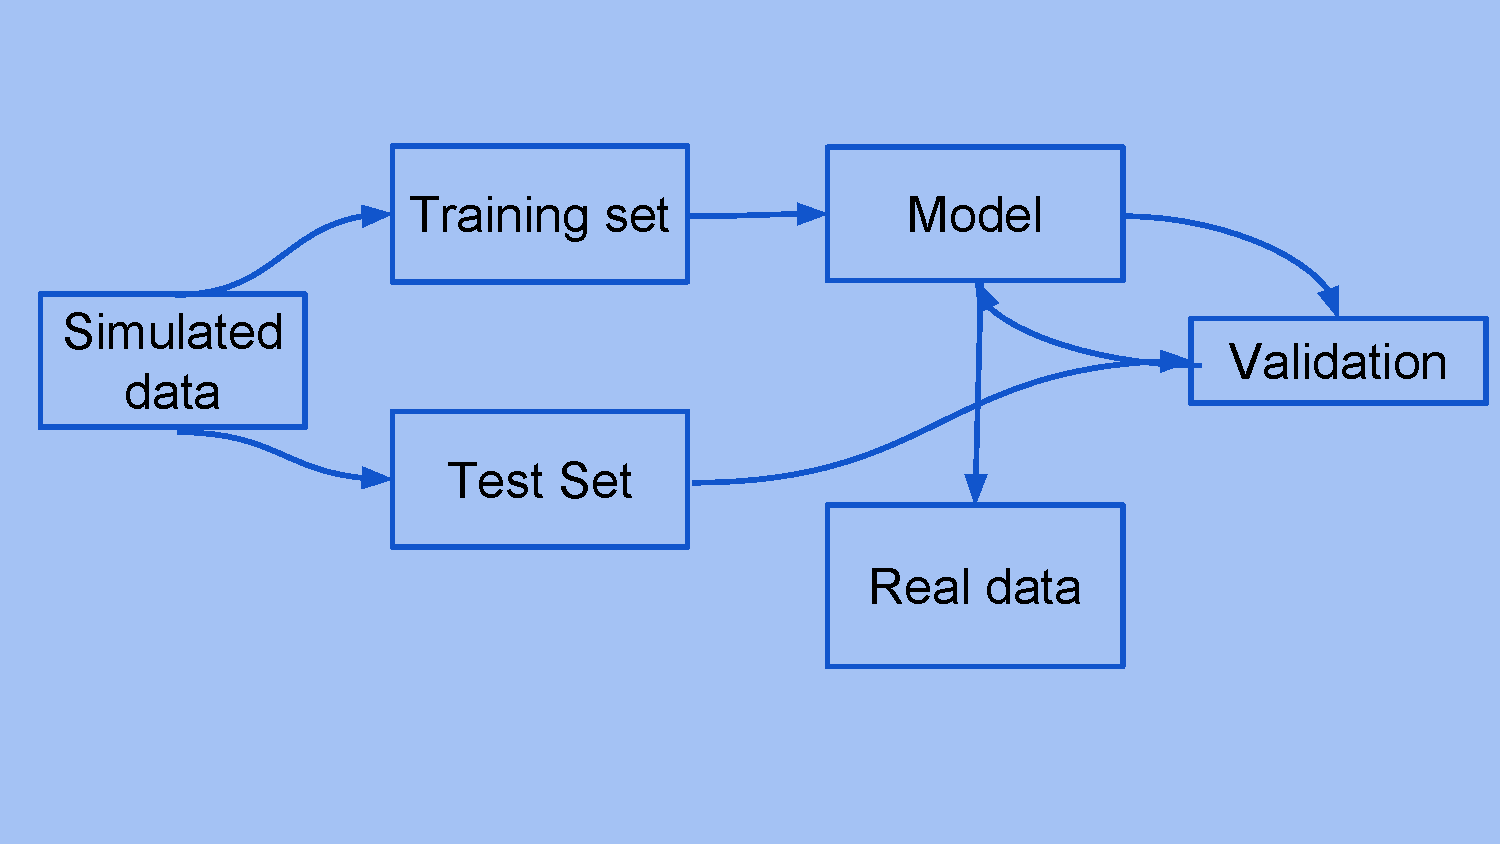
\includegraphics[scale=0.45]{./aprendizaje_supervisado.pdf}
  \end{center}
}

\begin{frame}
 \begin{figure}[ht!]
 \centering
 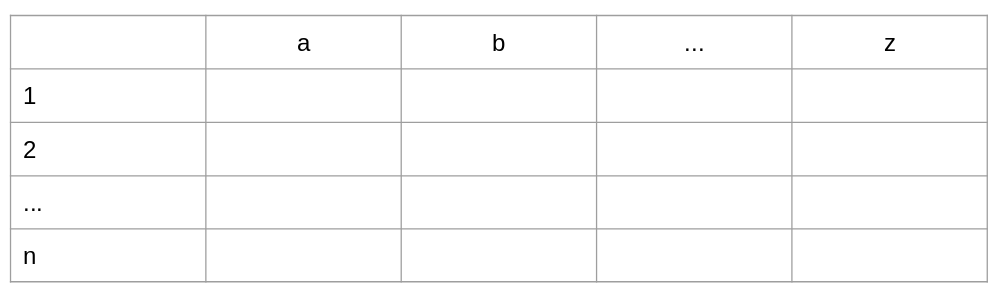
\includegraphics[scale=0.3]{table1.png}
 % table1.png: 1003x303 px, 72dpi, 35.38x10.69 cm, bb=0 0 1003 303
\end{figure}

\end{frame}

\begin{frame}
 \begin{figure}[ht!]
 \centering
 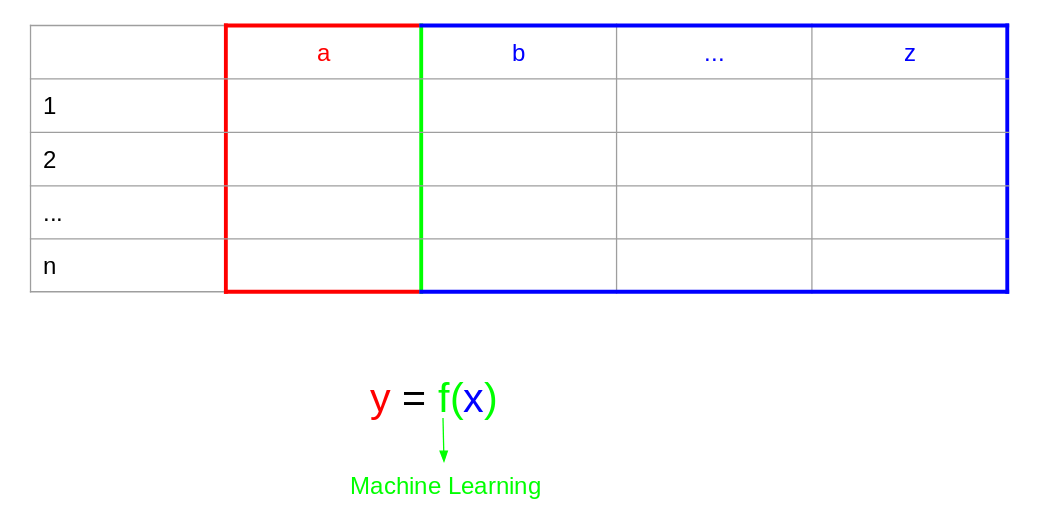
\includegraphics[scale=0.3]{table2.png}
 % table1.png: 1003x303 px, 72dpi, 35.38x10.69 cm, bb=0 0 1003 303
\end{figure}
\end{frame}

\begin{frame}
\begin{figure}[ht!]
 \centering
 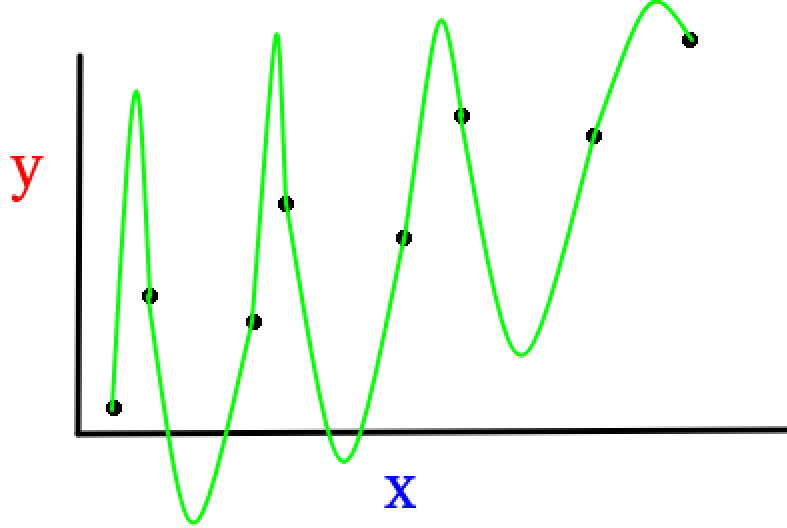
\includegraphics[scale=0.3]{f1.png}
 % f1.png: 787x528 px, 72dpi, 27.76x18.63 cm, bb=0 0 787 528
\end{figure}
\end{frame}

\begin{frame}
 \begin{figure}[ht!]
 \centering
 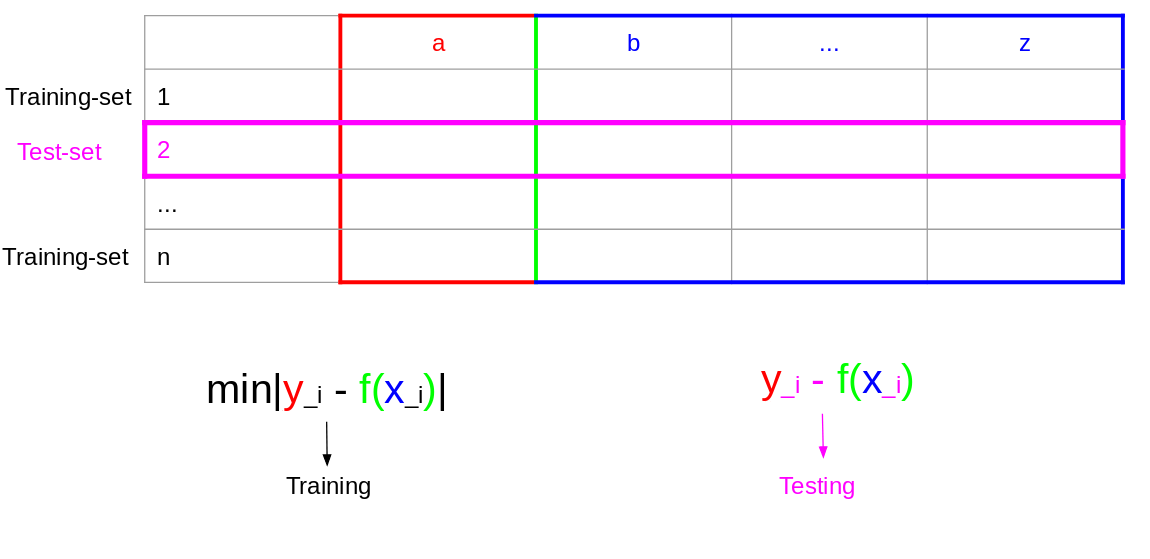
\includegraphics[scale=0.3]{table3.png}
 % table1.png: 1003x303 px, 72dpi, 35.38x10.69 cm, bb=0 0 1003 303
\end{figure}
\end{frame}

\begin{frame}
\begin{figure}[ht!]
 \centering
 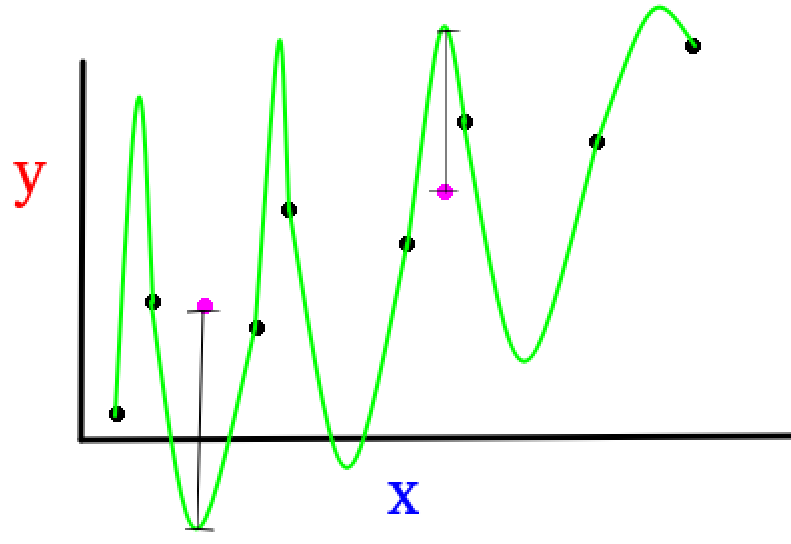
\includegraphics[scale=0.3]{f2.png}
 % f1.png: 787x528 px, 72dpi, 27.76x18.63 cm, bb=0 0 787 528
\end{figure}
\end{frame}

\begin{frame}
\begin{figure}[ht!]
 \centering
 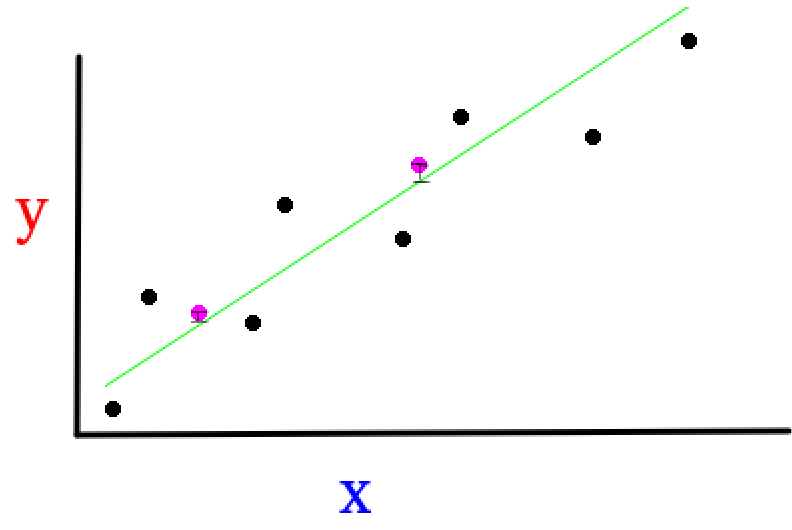
\includegraphics[scale=0.3]{f3.png}
 % f1.png: 787x528 px, 72dpi, 27.76x18.63 cm, bb=0 0 787 528
\end{figure}
\end{frame}

\begin{frame}
 \begin{figure}[ht!]
 \centering
 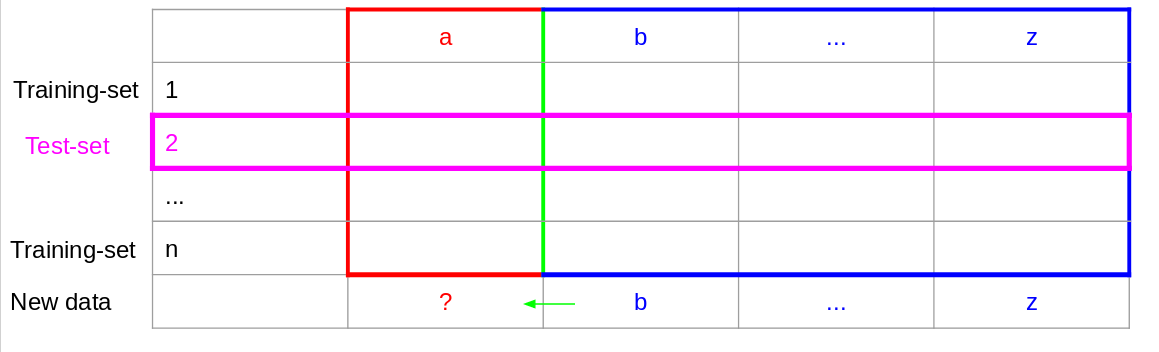
\includegraphics[scale=0.28]{table4.png}
 % table1.png: 1003x303 px, 72dpi, 35.38x10.69 cm, bb=0 0 1003 303
\end{figure}
\end{frame}

\subsection{Some important methods.}
\frame{
\tableofcontents[ 
    currentsubsection, 
    sectionstyle=show/hide, 
    sectionstyle=show/shaded, 
    ] 
}

\begin{frame}{Random Forest}
\begin{center}
  \animategraphics[loop,controls,scale=0.5]{5}{random_forest-}{0}{20}
\end{center}
\end{frame}

%\frame{
%  \frametitle{Random Forest}
%  \begin{center}
% 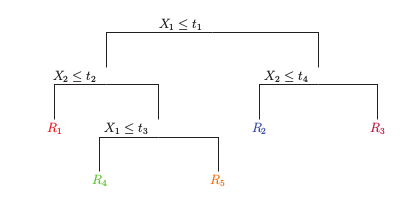
\includegraphics[scale=0.85]{./rf.png}
 % rf.png: 0x0 pixel, 300dpi, 0.00x0.00 cm, bb=
%\end{center}

%}

\begin{frame}{Support Vector Machines}
\begin{center}
  \animategraphics[loop,controls,scale=0.3]{10}{support_vector_machines-}{0}{40}
\end{center}
\end{frame}

\begin{frame}
 \begin{figure}[ht!]
 \centering
 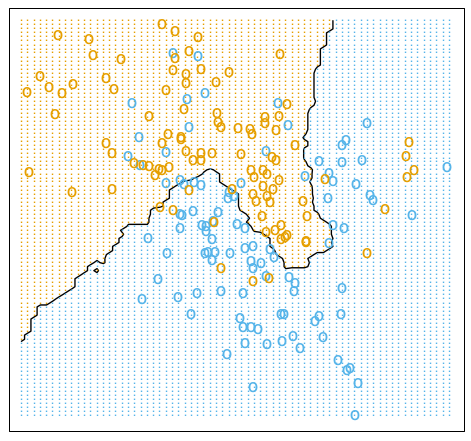
\includegraphics[scale=0.5]{knn.png}
 % knn.png: 471x441 px, 72dpi, 16.62x15.56 cm, bb=0 0 471 441
\end{figure}

\end{frame}

%\frame{
%  \frametitle{Support Vector Machine}
%  \begin{center}
% 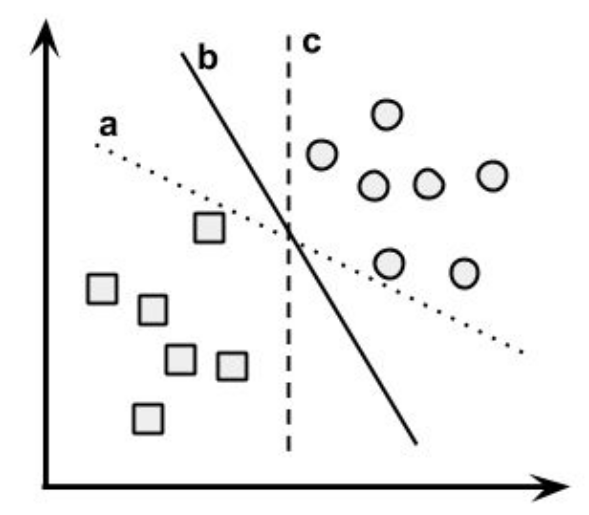
\includegraphics[scale=0.4]{./svm.png}

 % svm.png: 0x0 pixel, 300dpi, 0.00x0.00 cm, bb=
%\end{center}
%}

\begin{frame}
 \frametitle{Deep Learning}
 \begin{figure}[ht!]
 \centering
 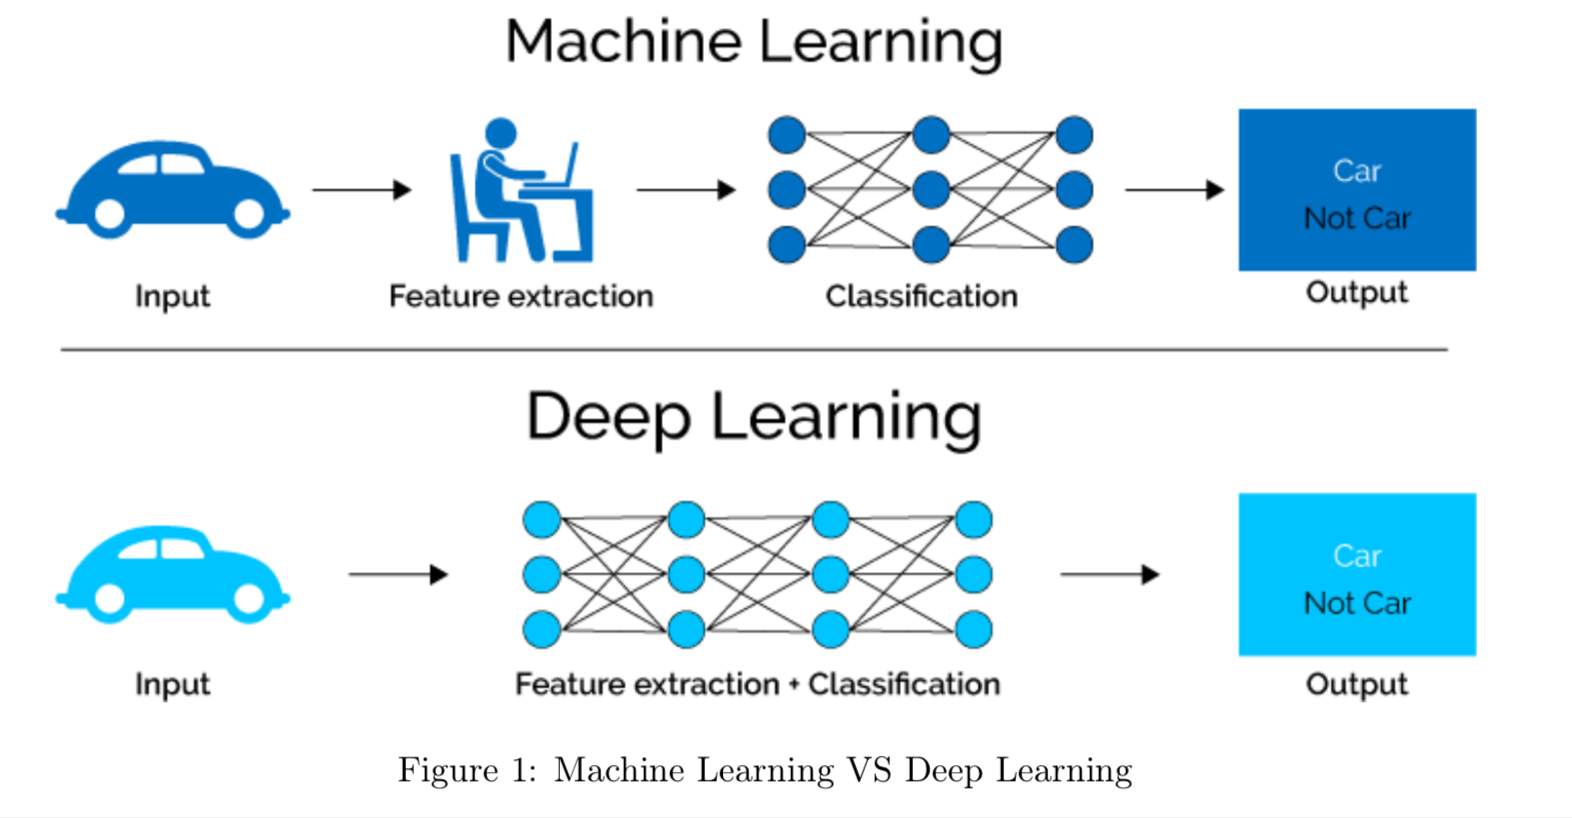
\includegraphics[scale=0.15]{deep.png}
 % deep.png: 960x540 px, 72dpi, 33.87x19.05 cm, bb=0 0 960 540
\end{figure}
\end{frame}


%\frame{
%  \frametitle{Unsupervised Learning.}
%  \begin{center}
% 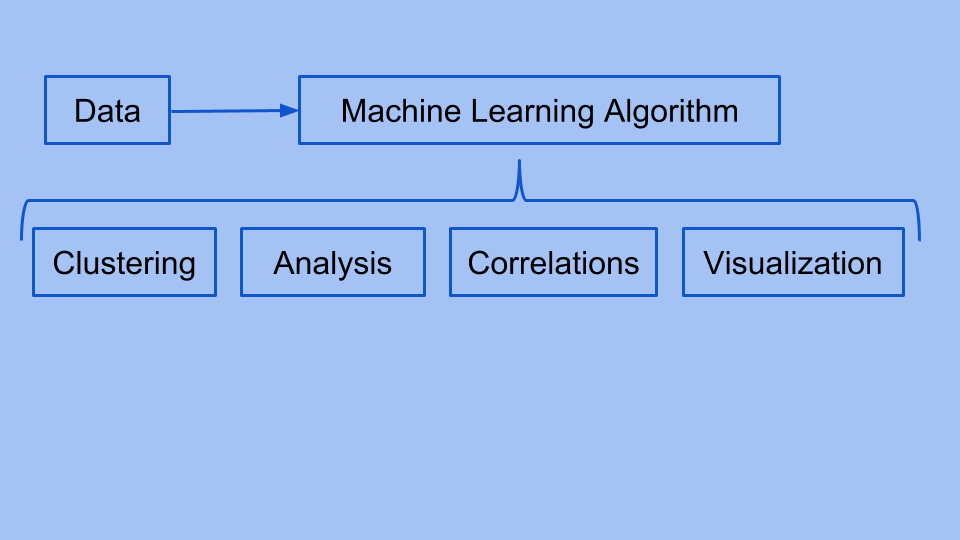
\includegraphics[scale=0.34]{./aprendizaje_nosupervisado.png}
 % aprendizaje_nosupervisado.jpg: 0x0 pixel, 300dpi, 0.00x0.00 cm, bb=
%\end{center}

%}


%\frame{
% \frametitle{Mixture of Gaussians.}
% \begin{center}
% 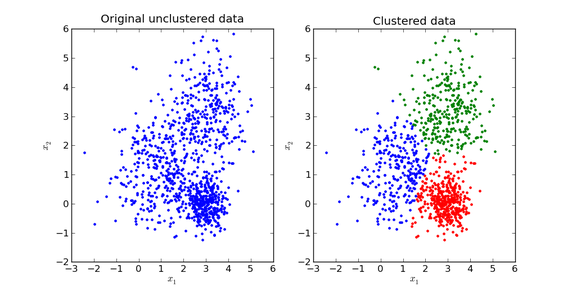
\includegraphics[scale=0.5]{./mixt_gauss.png}
 % mixt_gauss.png: 0x0 pixel, 300dpi, 0.00x0.00 cm, bb=
%\end{center}
%}

%\frame{
%\frametitle{Principal Components Analysis.}
%\begin{center}
% 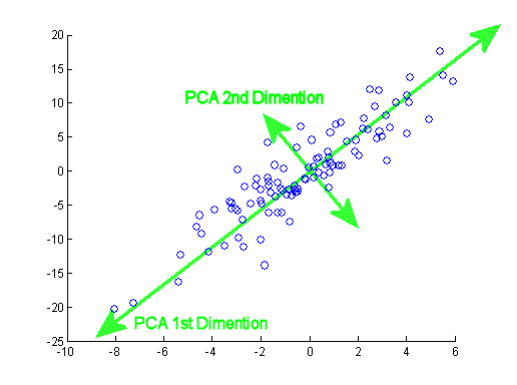
\includegraphics[scale=0.5]{./pca.png}
 % pca_example.gif: 0x0 pixel, 300dpi, 0.00x0.00 cm, bb=
%\end{center}
%}


%\begin{frame}{Mixture of Gaussians}
%\begin{center}
%  \animategraphics[loop,controls,scale=0.5]{5}{mixture_of_gaussians-}{0}{14}
%\end{center}
%\end{frame}

\subsection{Machine Learning in Astronomy.}
\frame{
\tableofcontents[ 
    currentsubsection, 
    sectionstyle=show/hide, 
    sectionstyle=show/shaded, 
    ] 
}

\begin{frame}
\frametitle{Classification Problems}
\begin{itemize}
 \item The S-PLUS: a star/galaxy classification based on a Machine Learning approach. {\color{azul}Costa-Duarte et al. (1909.08626)}
 \item A Neural Network Gravitational Arc Finder based on the Mediatrix filamentation Method. {\color{azul} Bom et al.  (1607.04644)}
 \item Circumventing Lens Modeling to Detect Dark Matter Substructure in Strong Lens
Images with Convolutional Neural Networks. {\color{azul}Diaz Rivero \& Dvorkin.  (1910.00015)}
 \item Distinguish standard and MOG with ML and weak
lensing. {\color{azul}Peel et al.  (1810.11030)}
\end{itemize}
\end{frame}

\begin{frame}
 \frametitle{Regression Problems}
 \begin{itemize}
  \item A Hybrid Deep Learning Approach to Cosmological Constraints From Galaxy Redshift Surveys.{\color{azul} Ntampaka et al.  (1909.10527)}
  \item An improved cosmological parameter inference scheme motivated by deep learning. {\color{azul} Ribli et al. (1806.05995)}
  \item Cosmological parameter estimation from large-scale structure deep learning. {\color{azul} Pan et al. (1908.10590)}
  \item Estimating Cosmological Parameters from the Dark Matter Distribution. {\color{azul} Ravanbakhsh et al. (1711.02033)}
 \end{itemize}

\end{frame}

\begin{frame}
 \frametitle{Other applications}
 \begin{itemize}
  \item CosmoGAN: creating high-fidelity weak lensing convergence maps using Generative Adversarial Networks. {\color{azul} Mustafa et al.  (1706.02390)}
  \item From Dark Matter to Galaxies with Convolutional Networks. {\color{azul} Zhang et al.  (1902.05965)}
  \item Learning to Predict the Cosmological Structure Formation.{\color{azul} He et al. (1811.06533)}
  \item CosmicNet I: Physics-driven implementation of neural networks within Boltzmann-Einstein solvers. {\color{azul} Albers et al.  (1907.05764)}
 \end{itemize}

\end{frame}

\section{The MeSsI Algorithm}
\frame{
\tableofcontents[ 
    currentsection, 
%    hideothersections, 
    sectionstyle=show/hide, 
    sectionstyle=show/shaded, 
    ] 
}

%\frame{
 %\frametitle{Other approachs for merging clusters detection}
 %\begin{columns}
  %\begin{column}{5cm}
   %Radio Haloes
  %\end{column}
  %\begin{column}{5cm}
   %X-ray morphologies
  %\end{column}
 %\end{columns}
%}

\frame{
 \begin{figure}[h!]
  \centering
  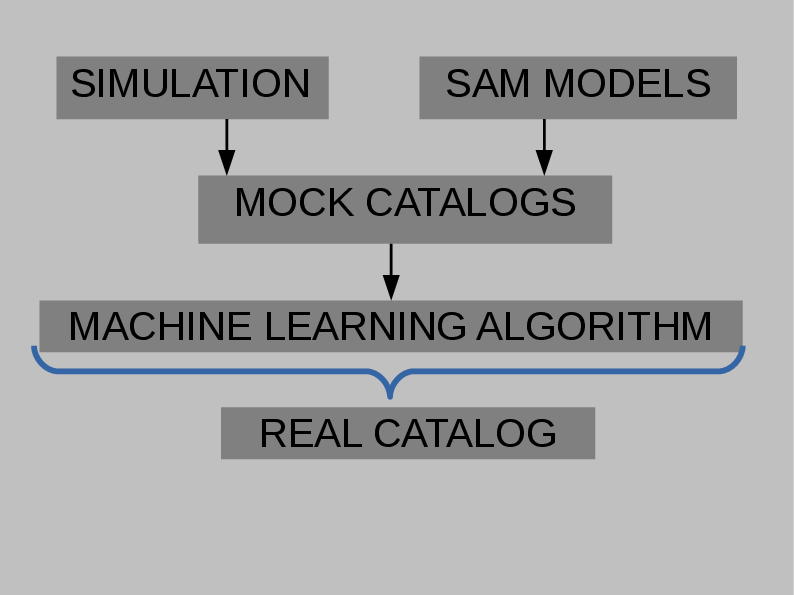
\includegraphics[scale=0.3]{./resu.png}
 % resu.pdf: 794x595 pixel, 72dpi, 28.01x20.99 cm, bb=0 0 794 595
 \end{figure}
}


\frame{ \frametitle{Clusters identification.}
\begin{itemize}
 \item We construct a mock catalogue based on the results of the application of the SAM Model of Guo et al. 2010
  to the Millenium simulation. \pause
 \item We Perform a friend-of-friend algorithm (\textit{Merchan \& Zandivares 2002 }) to the mock catalog in order to identify
  the clusters. \pause
 \item We assign each identified cluster with a fof-group in the simulation.
\end{itemize}
}

\frame{\frametitle{Study of the merger trees.}
 \begin{itemize}
  \item Based on the subhalos merger trees, we study the merger tree for every galaxy cluster in the mock catalog.
 \end{itemize}
 \begin{figure}[h!]
  \centering
  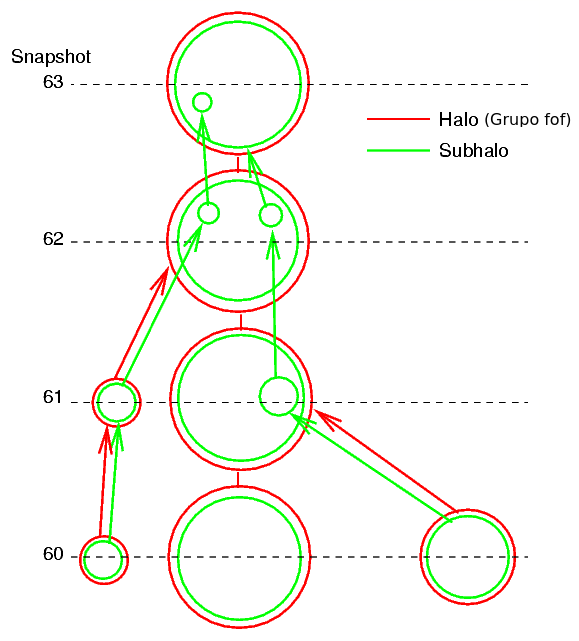
\includegraphics[scale=0.32]{./tree.png}
 % tree.eps: 0x0 pixel, 300dpi, 0.00x0.00 cm, bb=14 14 554 655
 \end{figure}
}

\subsection{Machine learning algorithm applied for identification of substructures.}
\frame{
\tableofcontents[ 
    currentsubsection, 
    sectionstyle=show/hide, 
    sectionstyle=show/shaded, 
    ] 
}

\frame{
 \begin{columns}
  \begin{column}{5cm}
   \begin{itemize}
    \item Dressler-Shectman test.
    \item Non gaussianity test.
    \item Color.
    \item Number of galaxies.
   \end{itemize}
  \end{column}
  \begin{column}{5cm}
   \begin{figure}[h!]
    \centering
    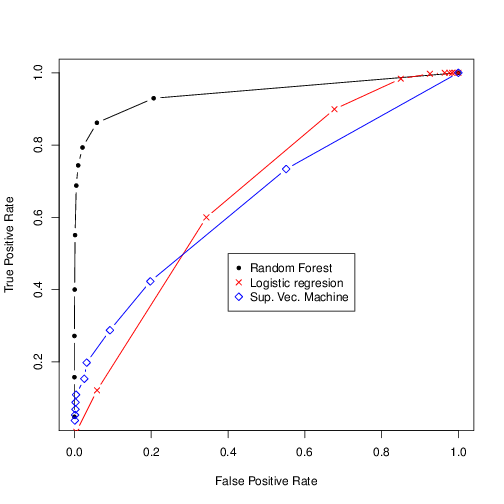
\includegraphics[scale=0.3]{./roc_curves.png}
    % roc_curves.pdf: 504x504 pixel, 72dpi, 17.78x17.78 cm, bb=0 0 504 504
   \end{figure}
  \end{column}
 \end{columns}
}

\frame{
\begin{figure}[h!]
 \centering
 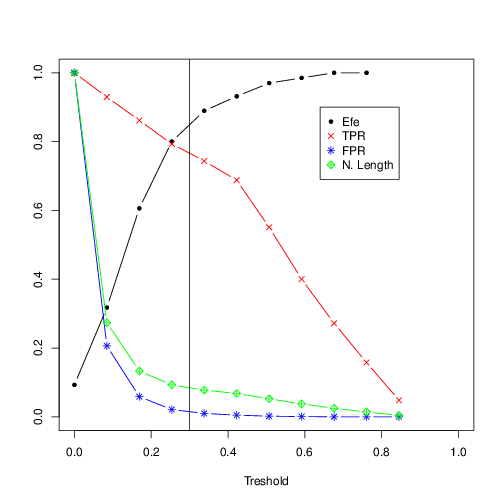
\includegraphics[scale=0.3]{./treshold.png}
 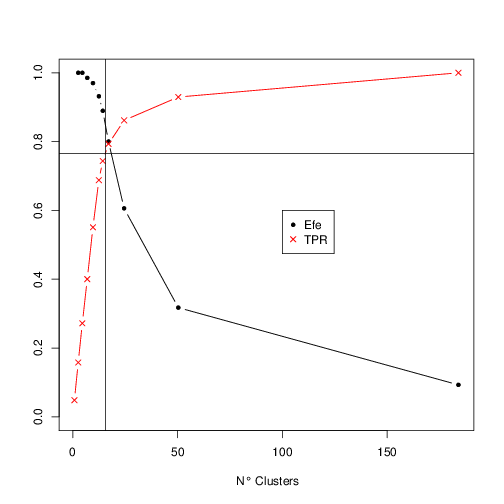
\includegraphics[scale=0.3]{./ncluster.png}
 % treshold.pdf: 504x504 pixel, 72dpi, 17.78x17.78 cm, bb=0 0 504 504
\end{figure}

}

\frame{
\frametitle{Study of the identified substructures.}
\begin{itemize}
 \item We ran a second stage of a random forest algorithm, applied to the galaxies. \pause
 \item In order to define substructures we identify clumps of galaxies based on their proximity, using a
  mixture of gaussians weighted by the probability of each galaxy of being part of a substructure, calculated
  with the RF. \pause
 \item After that, we estimate the velocity dispersion and the virial radius.

\end{itemize}
}

\frame{
 \frametitle{Application of the MeSsI Algorithm to spectroscopy catalogues}
  \begin{itemize}
   \item We find 12 Clusters with high probability of been in a merger in the SDSS DR7. \pause
   \item We find 7 Clusters with high probability of been in a merger in the WINGS Clusters. \pause
   \item We find 15 Clusters with high probability of been in a merger in the HECs Clusters.
  \end{itemize}

}

\begin{frame}
\href{https://github.com/Martindelosrios/MeSsI}{https://github.com/Martindelosrios/MeSsI}
\begin{figure}[ht!]
 \centering
 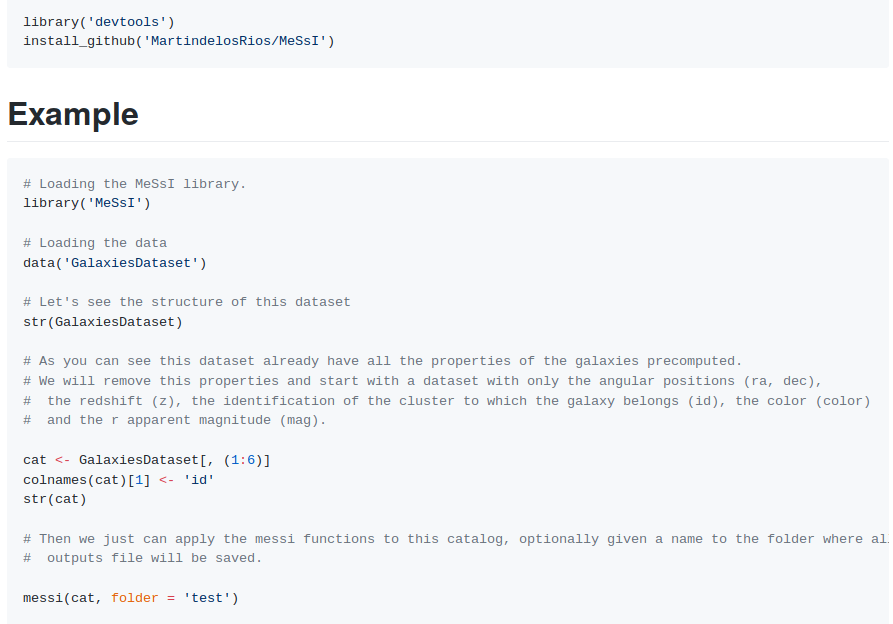
\includegraphics[scale=0.3]{messi_example.png}
 % messi_example.png: 893x624 px, 72dpi, 31.50x22.01 cm, bb=0 0 893 624
\end{figure}

\end{frame}


\subsection{A2029/2033 \& A1204.}
\frame{
\tableofcontents[ 
    currentsubsection, 
    sectionstyle=show/hide, 
    sectionstyle=show/shaded, 
    ] 
}

\frame{
\begin{figure}[ht!]
 \centering
 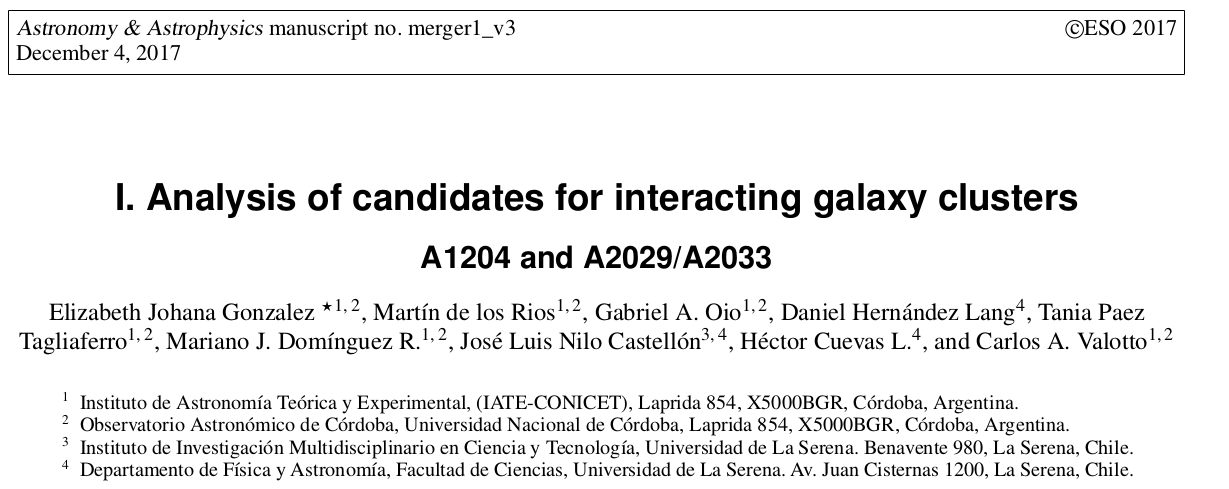
\includegraphics[scale=0.25]{a2029_paper.png}
 % a2029_paper.png: 1094x200 px, 96dpi, 28.94x5.29 cm, bb=0 0 820 150
\end{figure}
}

\frame{
\begin{center}
A2029/2033
\end{center}
\begin{figure}[ht!]
 \centering
 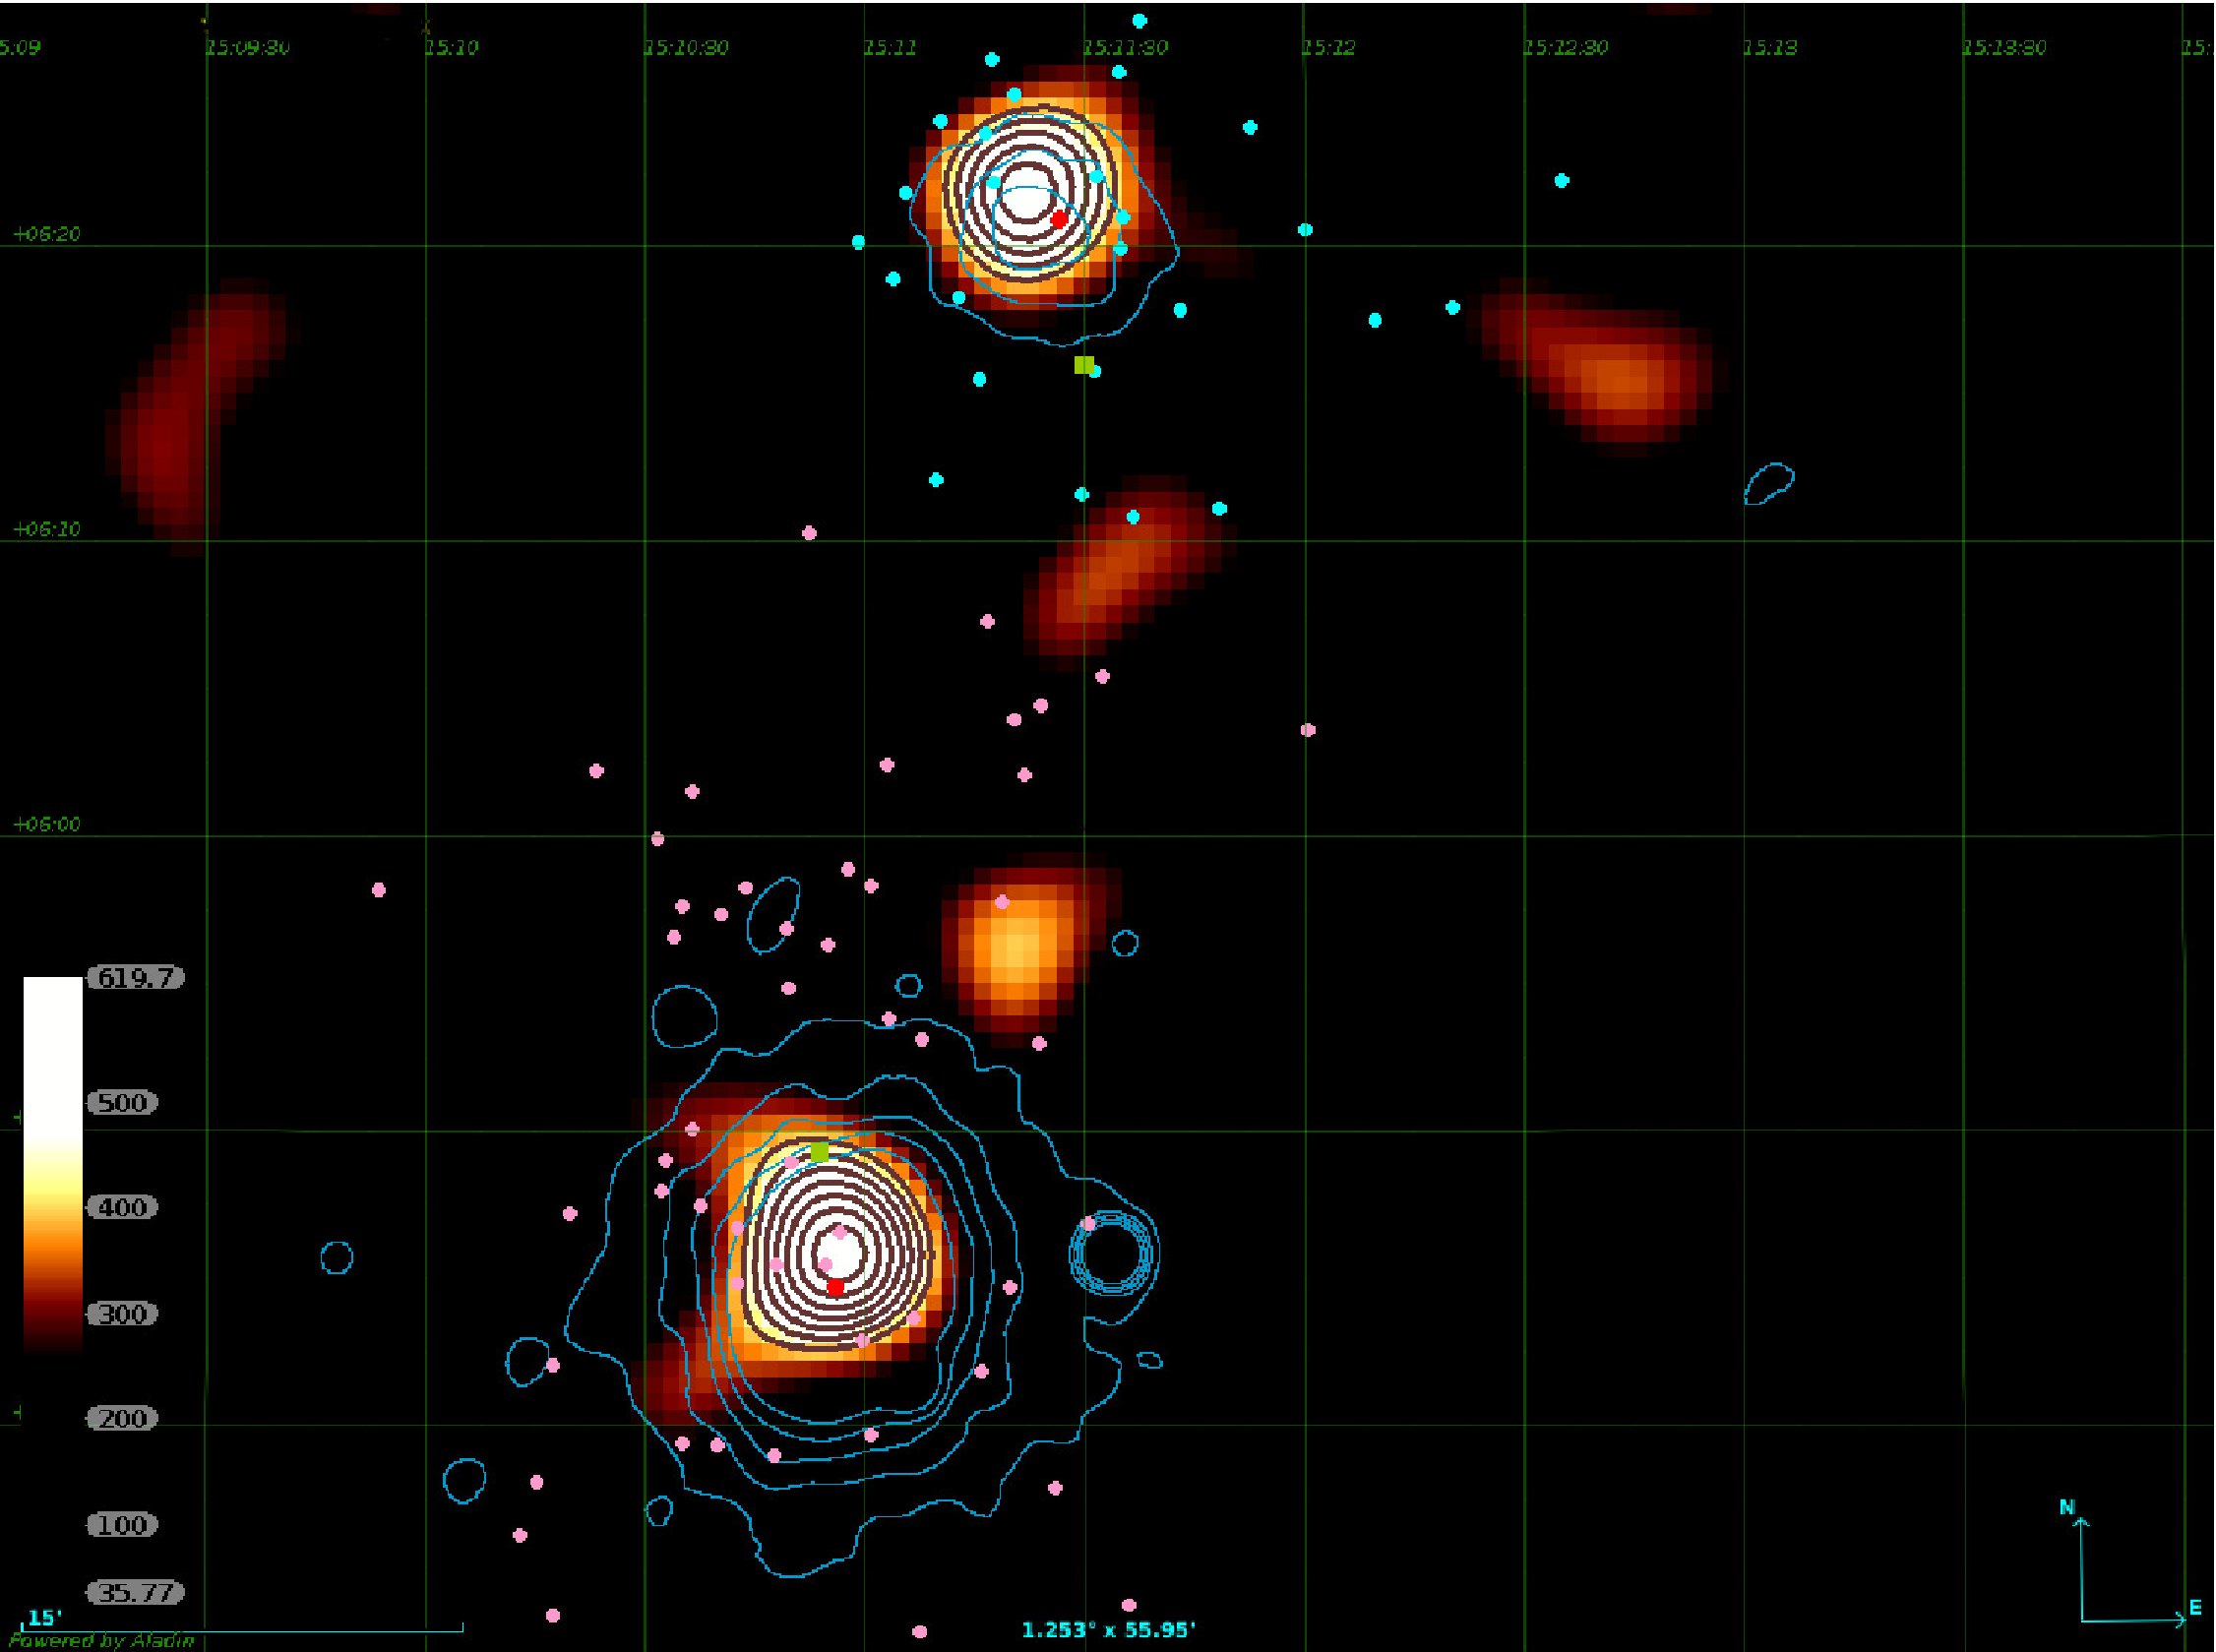
\includegraphics[scale=0.25]{A2029-2033-eps-converted-to.pdf}
 % A2029-2033-eps-converted-to.pdf: 0x0 px, 300dpi, 0.00x0.00 cm, bb=
\end{figure}

}
\subsection{A1204.}

\frame{
\begin{center}
A1204
\end{center}
\begin{figure}[ht!]
 \centering
 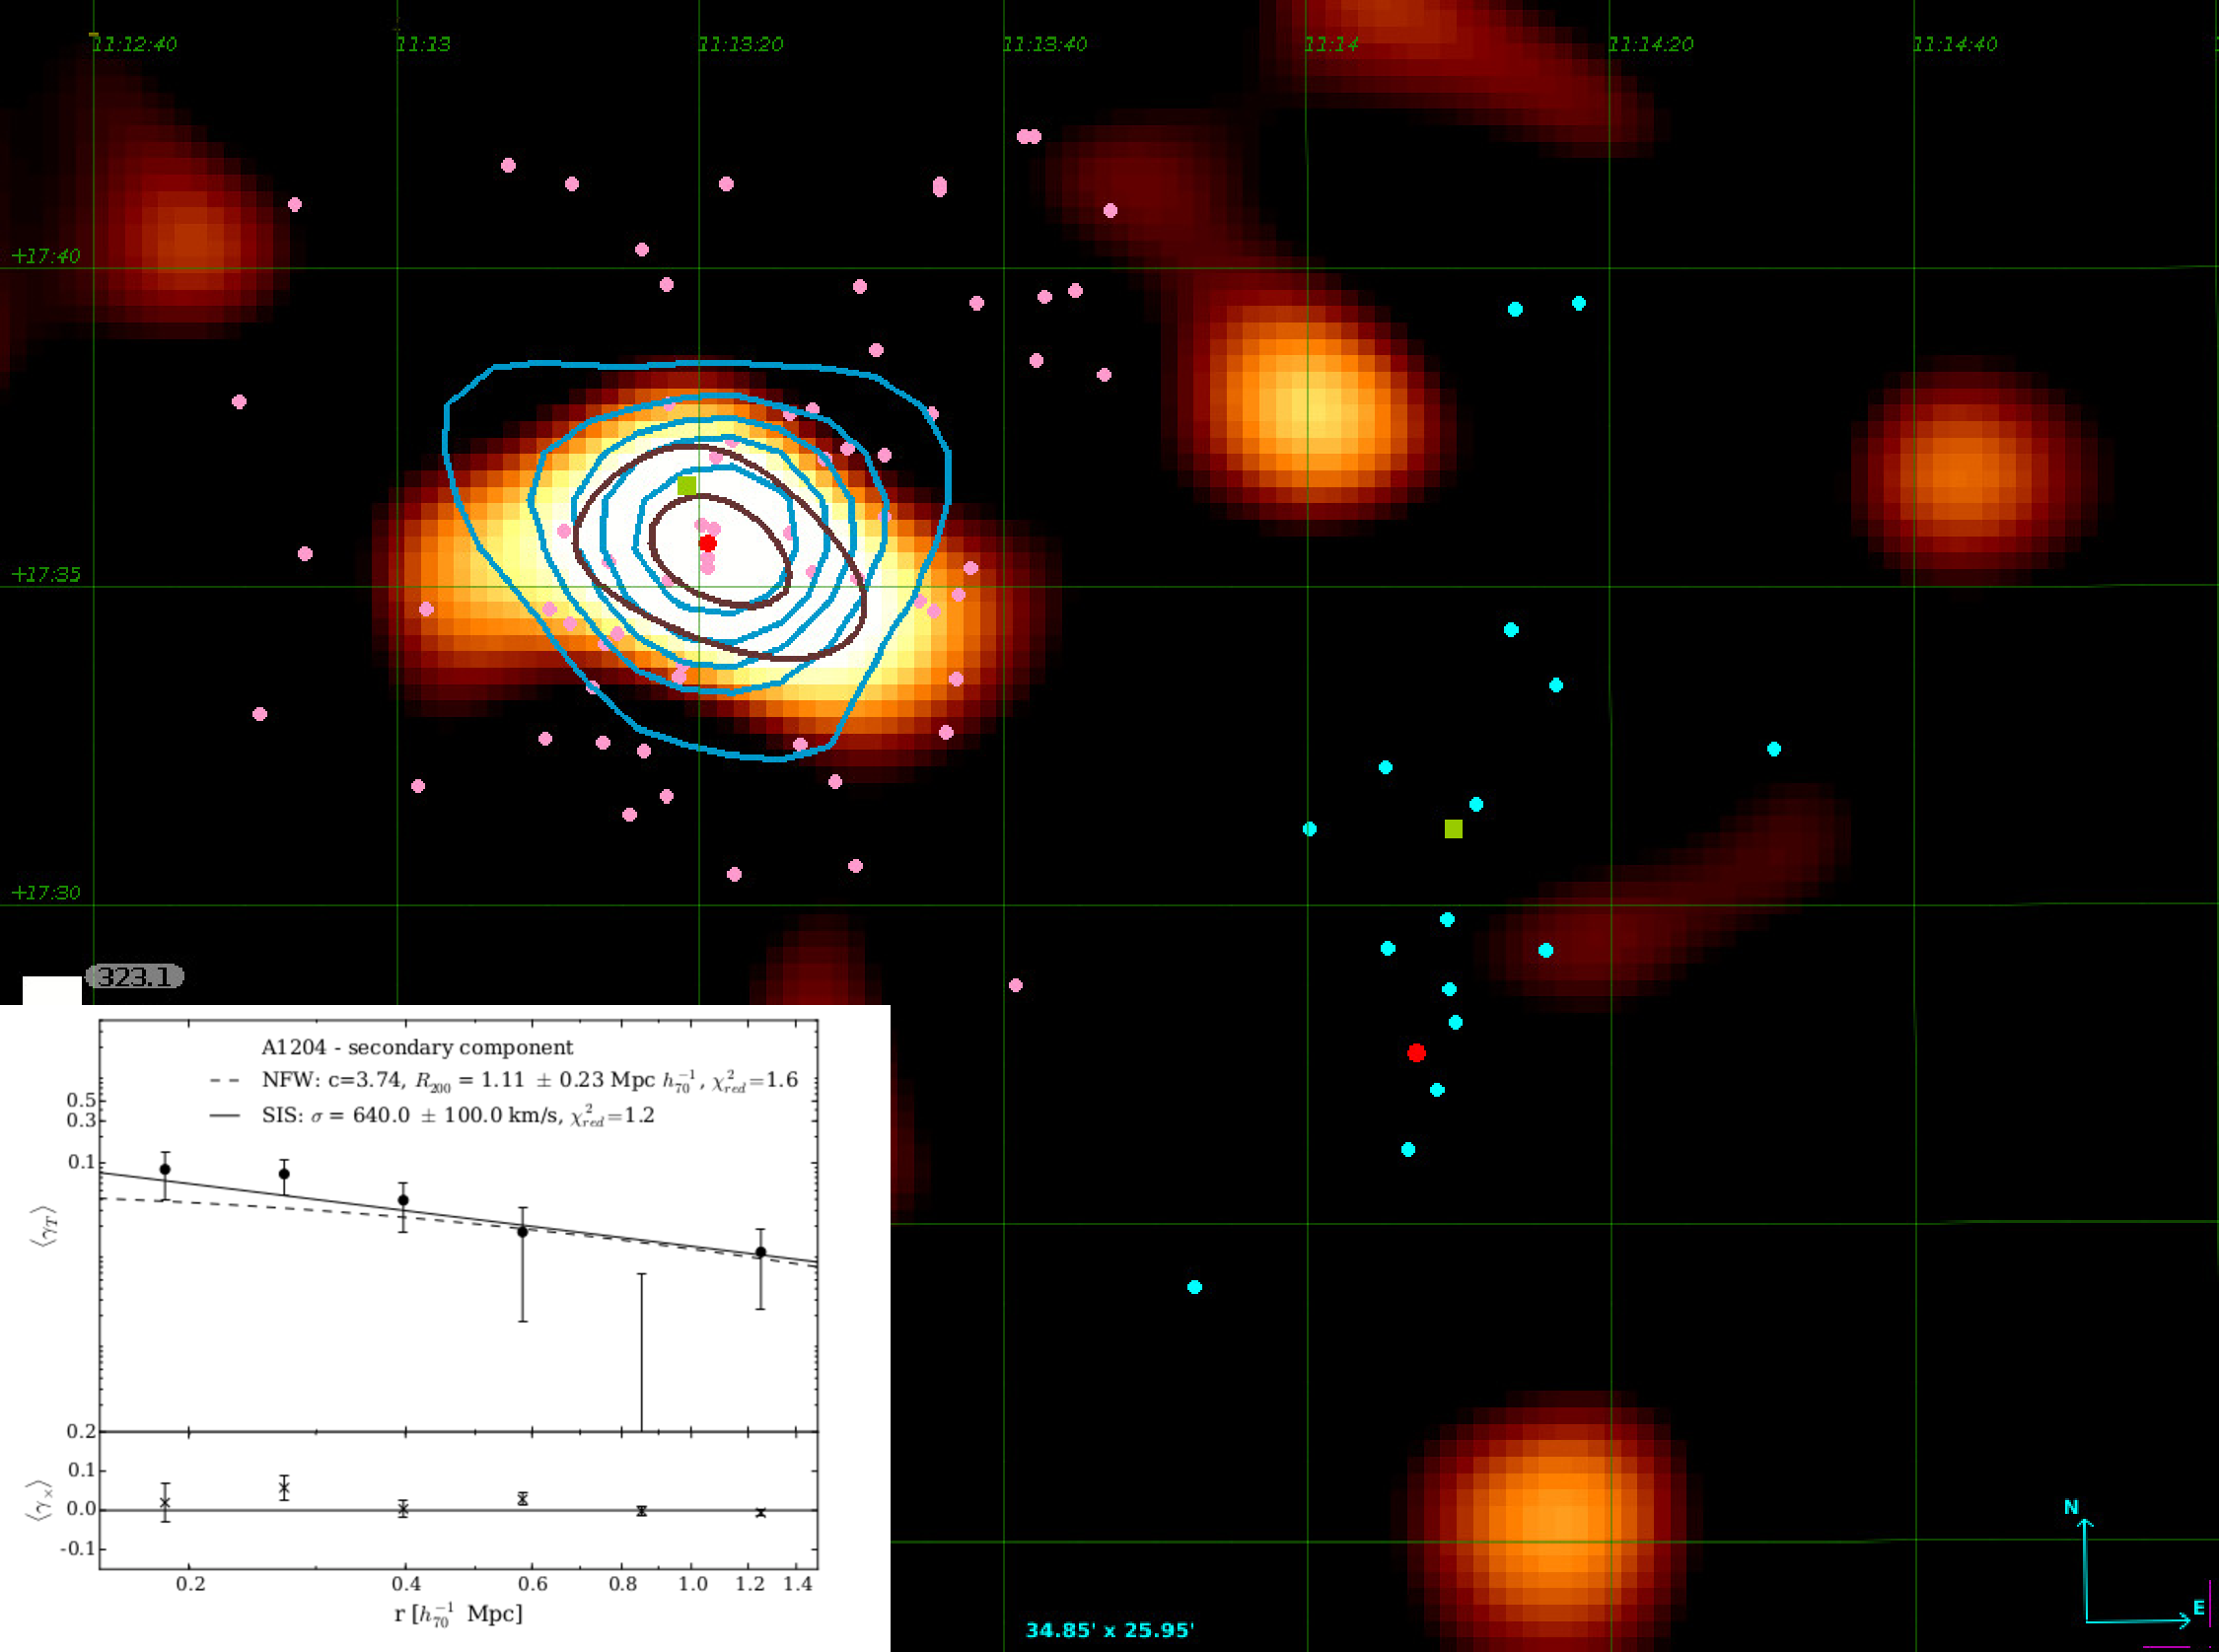
\includegraphics[scale=0.25]{A1204-eps-converted-to.pdf}
 % A1204-eps-converted-to.pdf: 0x0 px, 300dpi, 0.00x0.00 cm, bb=
\end{figure}
}
\subsection{A267.}
\frame{
\tableofcontents[ 
    currentsubsection, 
    sectionstyle=show/hide, 
    sectionstyle=show/shaded, 
    ] 
}
\frame{
\begin{figure}[ht!]
 \centering
 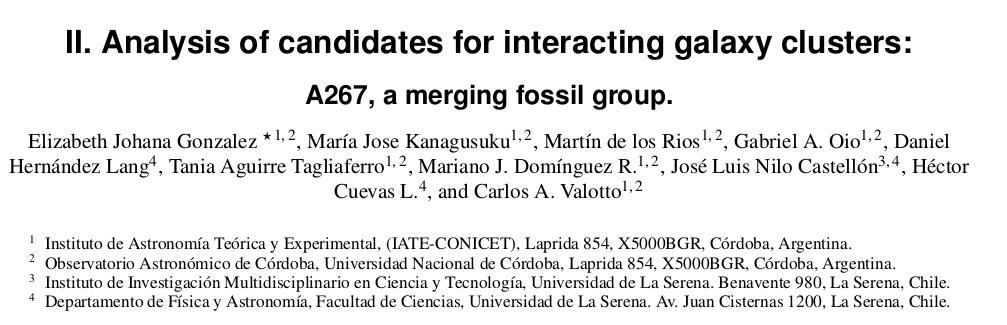
\includegraphics[scale=0.32]{a267_paper.png}
 % a2029_paper.png: 1094x200 px, 96dpi, 28.94x5.29 cm, bb=0 0 820 150
\end{figure}
}
\frame{
\begin{figure}[ht!]
 \centering
 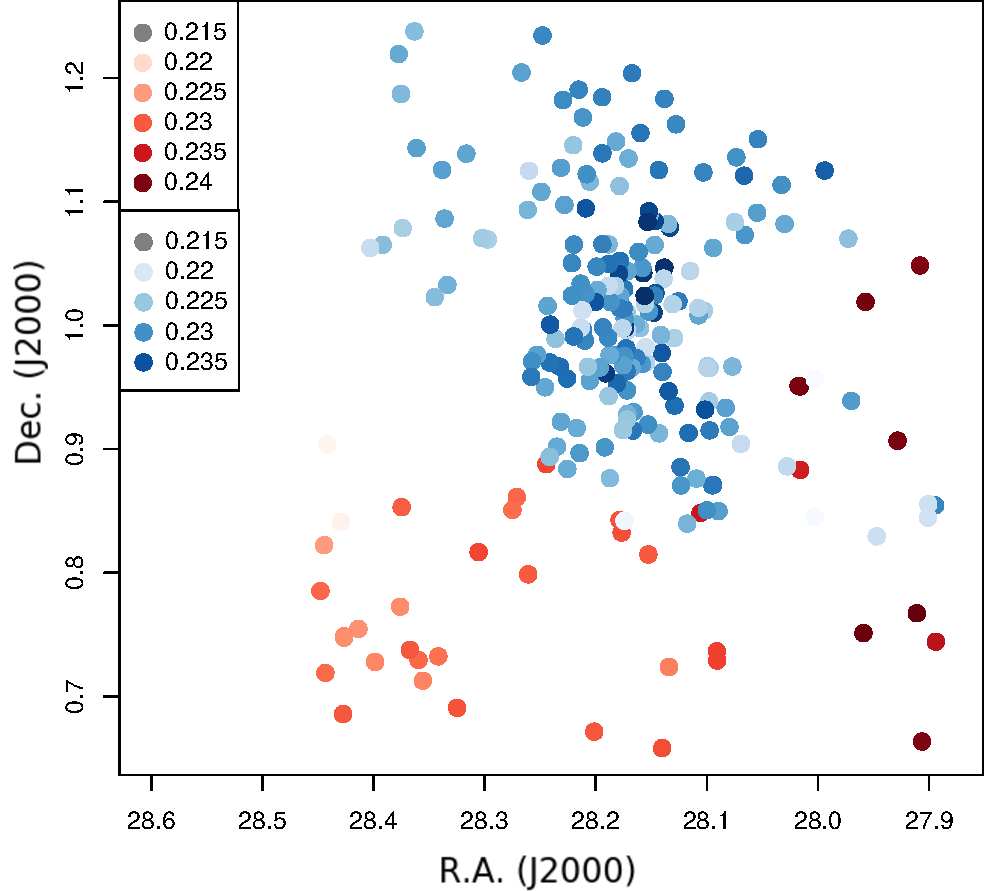
\includegraphics[scale=0.28]{redshift_angular.pdf}
 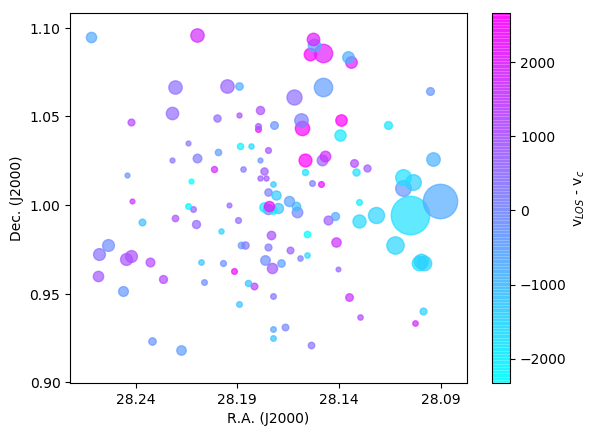
\includegraphics[scale=0.37]{dstest_a267_1.png}
 % redshift_angular.pdf: 0x0 px, 300dpi, 0.00x0.00 cm, bb=
\end{figure}
}
\frame{
\begin{columns}
  \begin{column}{5cm}
    \begin{figure}[ht!]
      \centering
        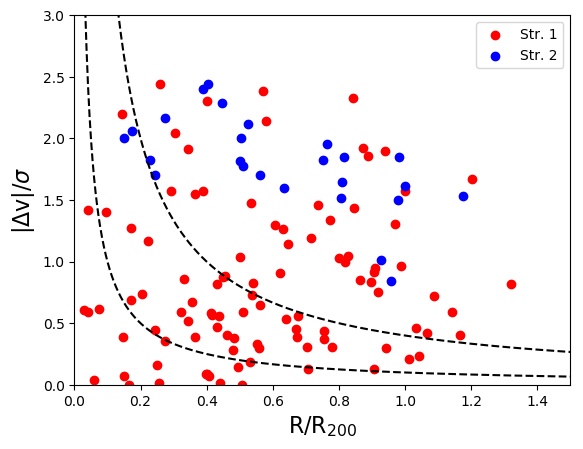
\includegraphics[scale=0.43]{a267_phasespace.png}
        %\includegraphics[scale=0.17]{fig_results2.eps}
    \end{figure}
    Noble et al. 2013
  \end{column}
  \begin{column}{5cm}
  \begin{itemize}
   \item $\approx 40\%$ Fossil groups have a major merger $z<0.8$.
   \item $\approx 15-25\%$ Fossil groups have a major merger $z<0.3$.
  \end{itemize}

  \end{column}
\end{columns}

}
\subsection{Statistical analysis of the magnetic fields in merging clusters.}
\frame{
\tableofcontents[ 
    currentsubsection, 
    sectionstyle=show/hide, 
    sectionstyle=show/shaded, 
    ] 
}
\frame{
\begin{figure}[ht!]
 \centering
 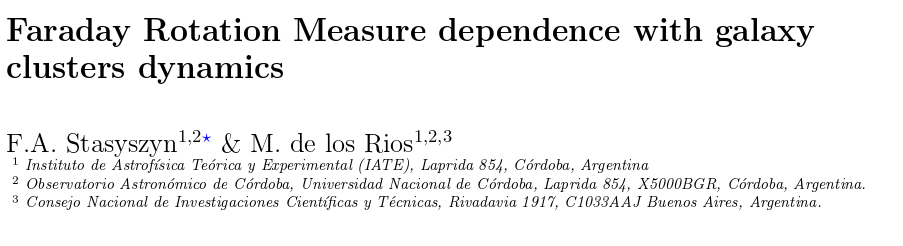
\includegraphics[scale=0.4]{magnetic_paper.png}
 % magnetic_paper.png: 710x230 px, 96dpi, 18.78x6.08 cm, bb=0 0 532 172
\end{figure}
}

\frame{
\begin{figure}[ht!]
 \centering
 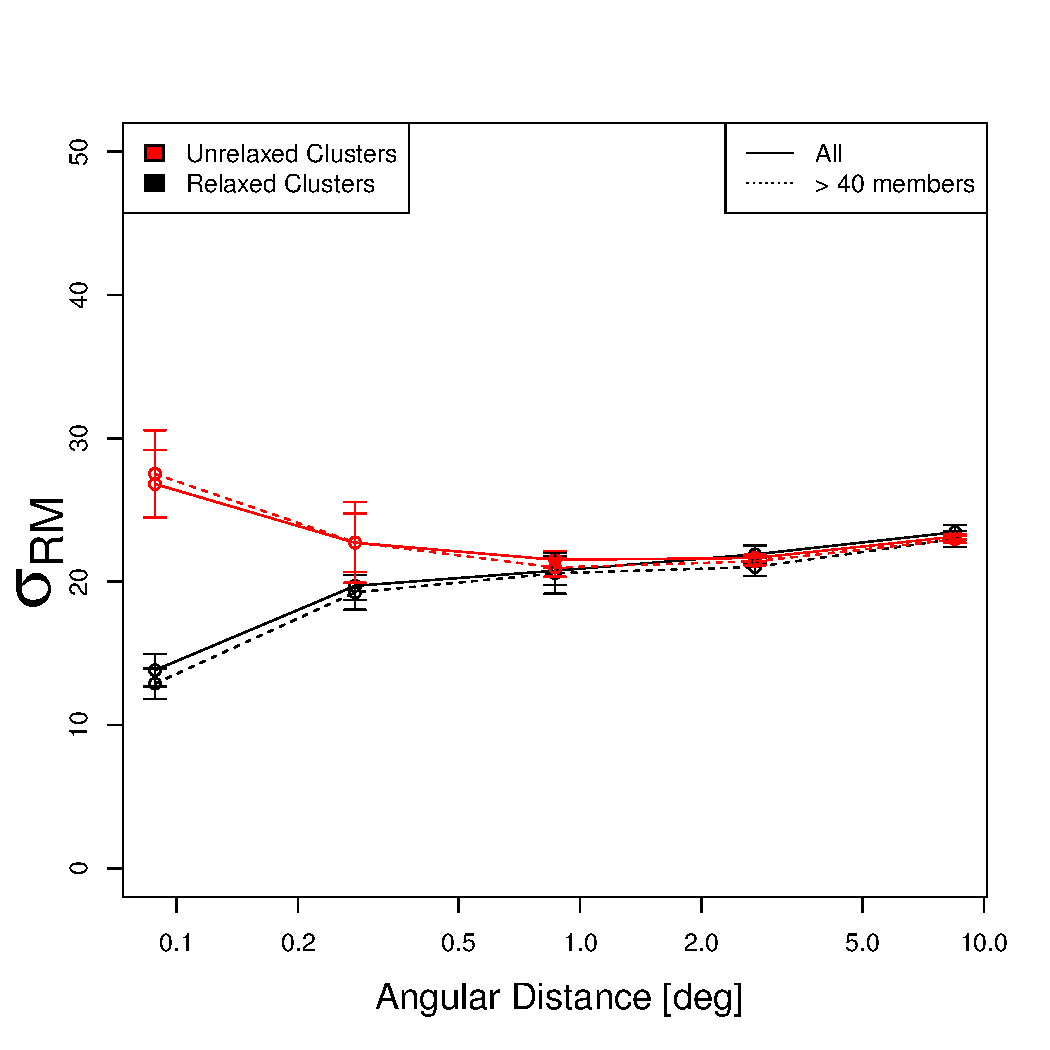
\includegraphics[scale=0.3]{AngTay01.pdf}
 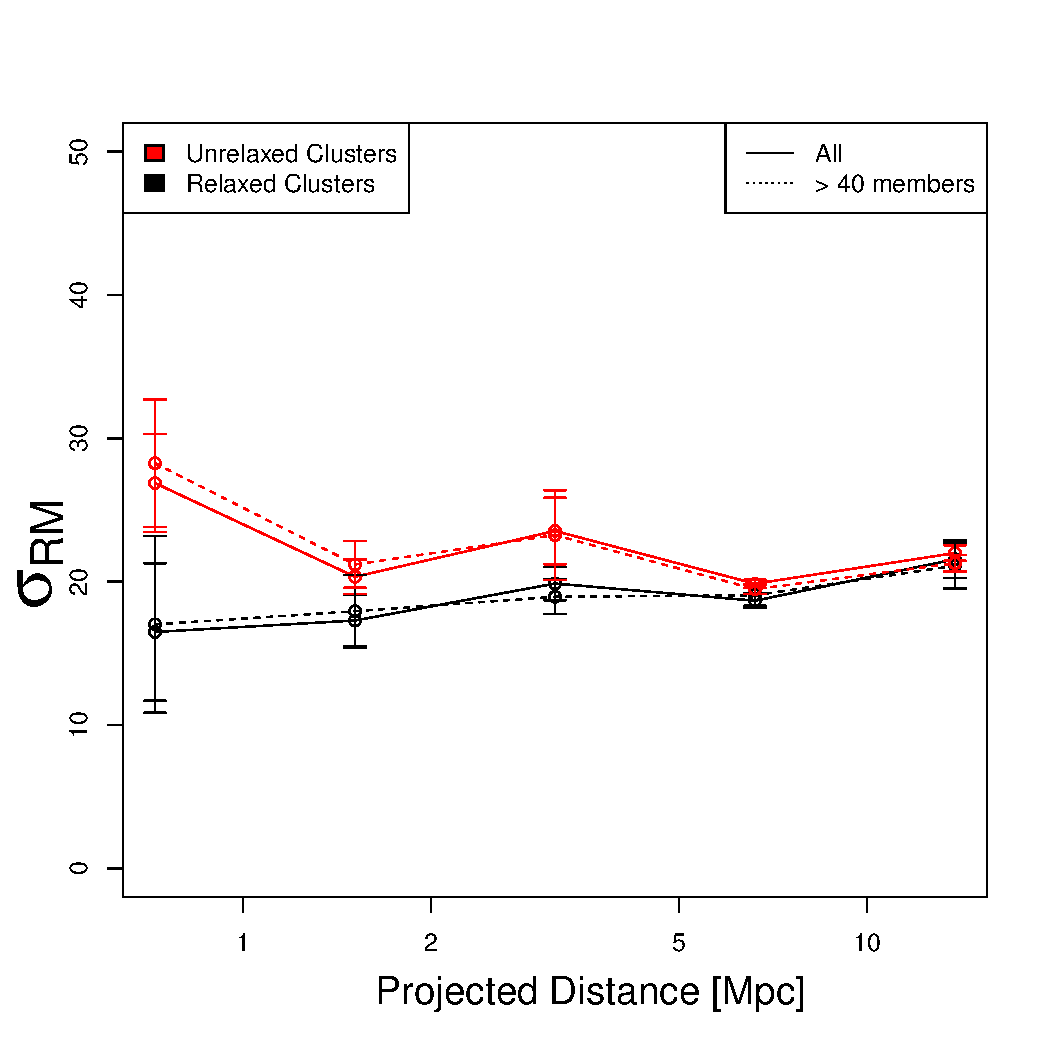
\includegraphics[scale=0.3]{ProTay01.pdf}
 % AngTay01.pdf: 0x0 px, 300dpi, 0.00x0.00 cm, bb=
\end{figure}

}

\section{DM-$\gamma$ interactions.}
\frame{
\tableofcontents[ 
    currentsubsection, 
    sectionstyle=show/hide, 
    sectionstyle=show/shaded, 
    ] 
}
\frame{\frametitle{DM-$\gamma$ interactions (work in progress)}
In collaboration with Dra. Celine B{\oe}hm
\begin{figure}[ht!]
 \centering
 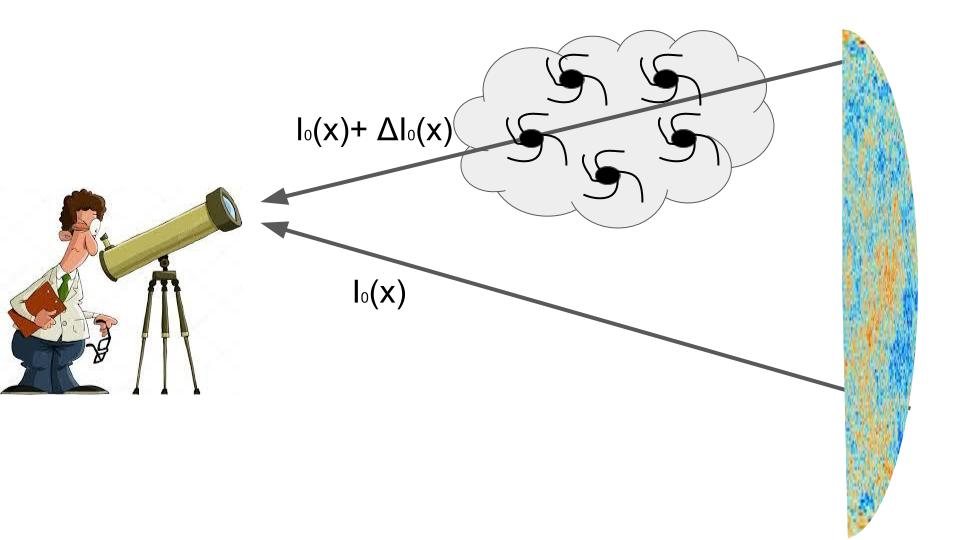
\includegraphics[scale=0.35]{./sz_effect.jpg}
 % sz_effect.jpg: 0x0 pixel, 300dpi, 0.00x0.00 cm, bb=
\end{figure}
}
\frame{
\begin{figure}[ht!]
 \centering
 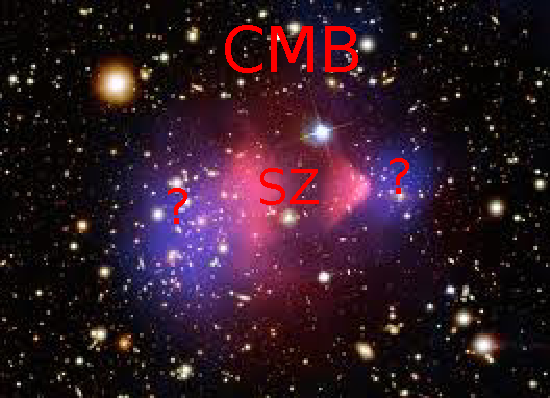
\includegraphics[scale=1.2]{gsz.pdf}
 % gsz.pdf: 0x0 px, 300dpi, 0.00x0.00 cm, bb=
\end{figure}

}

\section{Future Work}
\frame{
\tableofcontents[ 
    currentsection, 
%    hideothersections, 
    sectionstyle=show/hide, 
    sectionstyle=show/shaded, 
    ] 
}
\frame{
 \frametitle{Future Work}
 \begin{itemize}
  \item Perform astrophysical test over our sample of colliding cluster candidates of the catalog looking for
 impose some constraints on dark matter particle properties.
 \item Study the physics properties of the galaxies that belong to the identified substructures.
 \item Construct a catalog of relaxed clusters in order to study the dark matter equation of state (Serra \& Dominguez 2011).
 \item Study the candidate to merging cluster A376 (HSC SUBARU Images).
 \end{itemize}
}

\frame{
 \frametitle{Future Work}
 \begin{itemize}
  \item Estimate the CMB Masked Bispectra using Machine Learning techniques.
  \item Estimate the Dark matter Distribution of spiral galaxies using Deep Learning.
  \item Identifying backsplash galaxies in the phase-space using Machine Learning.
 \end{itemize}
}

\frame{ 
\begin{figure}[h!]
 \centering
 
\includegraphics[scale=0.4]{./gracias2.png}
 % gracias.png: 657x518 pixel, 72dpi, 23.18x18.27 cm, bb=0 0 657 518
\end{figure}
}
\end{document}

